\documentclass[11pt]{article}
\usepackage[margin=1.1in]{geometry}
\usepackage{amsmath,amssymb,amsthm}
\usepackage{booktabs}
\usepackage{tikz}
\usetikzlibrary{arrows.meta,positioning}
\usepackage[hidelinks]{hyperref}

\newtheorem{theorem}{Theorem}
\newtheorem{lemma}{Lemma}
\newtheorem{corollary}{Corollary}
\newtheorem{proposition}{Proposition}
\newtheorem{conjecture}{Conjecture}
\theoremstyle{definition}
\newtheorem{definition}{Definition}
\theoremstyle{remark}
\newtheorem{remark}{Remark}

\newcommand{\Sd}[2]{S_{#1}(#2)}
\newcommand{\NN}{\mathbb{N}}

\title{The Impossibility Spectrum of Shestoku:\\ \Large The Solvable Set Is Finite}
\author{Yosef A. Harris\\ \small shestoku.com}
\date{July 2026}

\begin{document}
\maketitle

\begin{abstract}
We study the $N$-flower Shestoku puzzle: $N$ disjoint seven-cell flowers are filled from the shared pool $\{1,\dots,7N\}$, each number used exactly once, subject to the rule that numbers on adjacent cells may neither be consecutive nor share a decimal digit. Intuition suggests that a larger board, offering a larger pool, can only become easier to fill; the small cases already refute this ($N=3,4,5$ are impossible), and the truth is far stronger: \emph{the set of solvable $N$ is finite}. We prove that the puzzle is impossible for every $N\ge 1514$, and more precisely that every $N$ outside the finite candidate set
\[
\mathcal{C} \;=\; \{1,2\}\;\cup\;[6,20]\;\cup\;[70,182]\;\cup\;[1387,1513]
\]
(257 values in all) admits an exact impossibility certificate. The engine is a hierarchy of counting obstructions built on the flower's unique maximum independent set: a generalized multi-digit saturation system, its linear relaxation, its Chv\'atal--Gomory rounding, a family of tier bounds that deduplicate multi-digit supply, and a class-flow refinement. The sporadic impossibilities $N=4,5$ are instances of the general mechanism, as are $N=51$, $67$ and $69$ --- values that successive drafts of this work had conjectured solvable, an in-house illustration of the paper's methodological thesis that plausible extrapolation is not proof. On the sufficiency side we verify solvability by explicit, independently checked constructions for every member of $\mathcal{C}$ outside the final window, so that the characterization is complete except on $[1387,1513]$; the residual conjecture is stated in exact and finite form.
\end{abstract}

\medskip
\noindent\textbf{Keywords:} number-placement puzzle; digit constraints; independent sets; integer programming certificates; Chv\'atal--Gomory rounding; combinatorial exhaustion.\\
\textbf{MSC 2020:} 00A08, 05C69, 11A63, 90C10.

\section{Introduction}

\subsection*{The puzzle, for the newcomer}

Shestoku is a pencil puzzle in the family of Sudoku and its kin, but built on hexagons rather than a square grid. Where Sudoku forbids a repeated \emph{symbol} in a row, Shestoku forbids a repeated \emph{digit} between neighbours: two cells that touch may not hold numbers that share any decimal digit, and --- a twist with no Sudoku analogue --- may not hold consecutive integers either. So $47$ and $71$ may not sit side by side (both contain a $7$), and neither may $47$ and $48$ (consecutive); but $47$ and $63$ are content neighbours. The solver's job is to place numbers so that every pair of touching cells is content.

The board is tiled by a repeating unit --- called an \emph{island} in the game, and a \emph{flower} throughout this paper --- consisting of seven hexagonal cells packed into the compact shape drawn in Figure~\ref{fig:flower}(a). Two cells are \emph{neighbours} when they share a border; the seven cells have ten such borders in all. One cell, the \emph{hub} (orange), borders four others, while the two outermost cells border only two each. A single flower therefore holds seven numbers subject to ten neighbour-constraints. Figure~\ref{fig:flower}(b) shows one legal way to fill a single flower with the numbers $1,\dots,7$: the reader may check that every pair of bordering cells holds numbers that neither share a digit nor run consecutively.

\begin{figure}[ht]
\centering
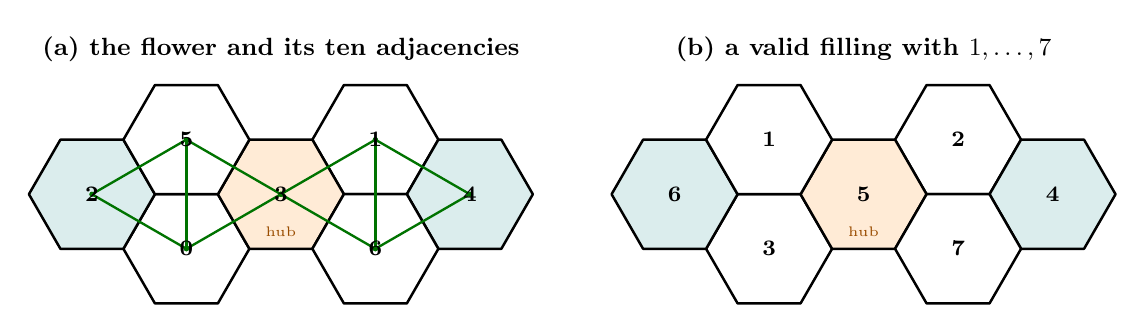
\begin{tikzpicture}[line join=round]
\begin{scope}[xshift=0.00cm]
\node[font=\bfseries\small] at (0,1.84) {(a) the flower and its ten adjacencies};
\fill[white] (-0.400,-0.693) -- (-0.800,0.000) -- (-1.600,0.000) -- (-2.000,-0.693) -- (-1.600,-1.386) -- (-0.800,-1.386) -- cycle;
\draw[black,line width=0.9pt] (-0.400,-0.693) -- (-0.800,0.000) -- (-1.600,0.000) -- (-2.000,-0.693) -- (-1.600,-1.386) -- (-0.800,-1.386) -- cycle;
\fill[white] (2.000,0.693) -- (1.600,1.386) -- (0.800,1.386) -- (0.400,0.693) -- (0.800,-0.000) -- (1.600,-0.000) -- cycle;
\draw[black,line width=0.9pt] (2.000,0.693) -- (1.600,1.386) -- (0.800,1.386) -- (0.400,0.693) -- (0.800,-0.000) -- (1.600,-0.000) -- cycle;
\fill[teal!14] (-1.600,0.000) -- (-2.000,0.693) -- (-2.800,0.693) -- (-3.200,0.000) -- (-2.800,-0.693) -- (-2.000,-0.693) -- cycle;
\draw[black,line width=0.9pt] (-1.600,0.000) -- (-2.000,0.693) -- (-2.800,0.693) -- (-3.200,0.000) -- (-2.800,-0.693) -- (-2.000,-0.693) -- cycle;
\fill[orange!16] (0.800,0.000) -- (0.400,0.693) -- (-0.400,0.693) -- (-0.800,0.000) -- (-0.400,-0.693) -- (0.400,-0.693) -- cycle;
\draw[black,line width=0.9pt] (0.800,0.000) -- (0.400,0.693) -- (-0.400,0.693) -- (-0.800,0.000) -- (-0.400,-0.693) -- (0.400,-0.693) -- cycle;
\fill[teal!14] (3.200,0.000) -- (2.800,0.693) -- (2.000,0.693) -- (1.600,0.000) -- (2.000,-0.693) -- (2.800,-0.693) -- cycle;
\draw[black,line width=0.9pt] (3.200,0.000) -- (2.800,0.693) -- (2.000,0.693) -- (1.600,0.000) -- (2.000,-0.693) -- (2.800,-0.693) -- cycle;
\fill[white] (-0.400,0.693) -- (-0.800,1.386) -- (-1.600,1.386) -- (-2.000,0.693) -- (-1.600,-0.000) -- (-0.800,-0.000) -- cycle;
\draw[black,line width=0.9pt] (-0.400,0.693) -- (-0.800,1.386) -- (-1.600,1.386) -- (-2.000,0.693) -- (-1.600,-0.000) -- (-0.800,-0.000) -- cycle;
\fill[white] (2.000,-0.693) -- (1.600,0.000) -- (0.800,0.000) -- (0.400,-0.693) -- (0.800,-1.386) -- (1.600,-1.386) -- cycle;
\draw[black,line width=0.9pt] (2.000,-0.693) -- (1.600,0.000) -- (0.800,0.000) -- (0.400,-0.693) -- (0.800,-1.386) -- (1.600,-1.386) -- cycle;
\draw[green!45!black,line width=0.85pt] (-1.200,-0.693) -- (-2.400,0.000);
\fill[green!45!black] (-1.200,-0.693) circle (0.9pt);
\fill[green!45!black] (-2.400,0.000) circle (0.9pt);
\draw[green!45!black,line width=0.85pt] (-1.200,-0.693) -- (0.000,0.000);
\fill[green!45!black] (-1.200,-0.693) circle (0.9pt);
\fill[green!45!black] (0.000,0.000) circle (0.9pt);
\draw[green!45!black,line width=0.85pt] (-1.200,-0.693) -- (-1.200,0.693);
\fill[green!45!black] (-1.200,-0.693) circle (0.9pt);
\fill[green!45!black] (-1.200,0.693) circle (0.9pt);
\draw[green!45!black,line width=0.85pt] (1.200,0.693) -- (0.000,0.000);
\fill[green!45!black] (1.200,0.693) circle (0.9pt);
\fill[green!45!black] (0.000,0.000) circle (0.9pt);
\draw[green!45!black,line width=0.85pt] (1.200,0.693) -- (2.400,0.000);
\fill[green!45!black] (1.200,0.693) circle (0.9pt);
\fill[green!45!black] (2.400,0.000) circle (0.9pt);
\draw[green!45!black,line width=0.85pt] (1.200,0.693) -- (1.200,-0.693);
\fill[green!45!black] (1.200,0.693) circle (0.9pt);
\fill[green!45!black] (1.200,-0.693) circle (0.9pt);
\draw[green!45!black,line width=0.85pt] (-2.400,0.000) -- (-1.200,0.693);
\fill[green!45!black] (-2.400,0.000) circle (0.9pt);
\fill[green!45!black] (-1.200,0.693) circle (0.9pt);
\draw[green!45!black,line width=0.85pt] (0.000,0.000) -- (-1.200,0.693);
\fill[green!45!black] (0.000,0.000) circle (0.9pt);
\fill[green!45!black] (-1.200,0.693) circle (0.9pt);
\draw[green!45!black,line width=0.85pt] (0.000,0.000) -- (1.200,-0.693);
\fill[green!45!black] (0.000,0.000) circle (0.9pt);
\fill[green!45!black] (1.200,-0.693) circle (0.9pt);
\draw[green!45!black,line width=0.85pt] (2.400,0.000) -- (1.200,-0.693);
\fill[green!45!black] (2.400,0.000) circle (0.9pt);
\fill[green!45!black] (1.200,-0.693) circle (0.9pt);
\node[font=\footnotesize\bfseries] at (-1.200,-0.693) {0};
\node[font=\footnotesize\bfseries] at (1.200,0.693) {1};
\node[font=\footnotesize\bfseries] at (-2.400,0.000) {2};
\node[font=\footnotesize\bfseries] at (0.000,0.000) {3};
\node[font=\footnotesize\bfseries] at (2.400,0.000) {4};
\node[font=\footnotesize\bfseries] at (-1.200,0.693) {5};
\node[font=\footnotesize\bfseries] at (1.200,-0.693) {6};
\node[font=\tiny,orange!60!black] at (0.000,-0.480) {hub};
\end{scope}
\begin{scope}[xshift=7.40cm]
\node[font=\bfseries\small] at (0,1.84) {(b) a valid filling with $1,\dots,7$};
\fill[white] (-0.400,-0.693) -- (-0.800,0.000) -- (-1.600,0.000) -- (-2.000,-0.693) -- (-1.600,-1.386) -- (-0.800,-1.386) -- cycle;
\draw[black,line width=0.9pt] (-0.400,-0.693) -- (-0.800,0.000) -- (-1.600,0.000) -- (-2.000,-0.693) -- (-1.600,-1.386) -- (-0.800,-1.386) -- cycle;
\fill[white] (2.000,0.693) -- (1.600,1.386) -- (0.800,1.386) -- (0.400,0.693) -- (0.800,-0.000) -- (1.600,-0.000) -- cycle;
\draw[black,line width=0.9pt] (2.000,0.693) -- (1.600,1.386) -- (0.800,1.386) -- (0.400,0.693) -- (0.800,-0.000) -- (1.600,-0.000) -- cycle;
\fill[teal!14] (-1.600,0.000) -- (-2.000,0.693) -- (-2.800,0.693) -- (-3.200,0.000) -- (-2.800,-0.693) -- (-2.000,-0.693) -- cycle;
\draw[black,line width=0.9pt] (-1.600,0.000) -- (-2.000,0.693) -- (-2.800,0.693) -- (-3.200,0.000) -- (-2.800,-0.693) -- (-2.000,-0.693) -- cycle;
\fill[orange!16] (0.800,0.000) -- (0.400,0.693) -- (-0.400,0.693) -- (-0.800,0.000) -- (-0.400,-0.693) -- (0.400,-0.693) -- cycle;
\draw[black,line width=0.9pt] (0.800,0.000) -- (0.400,0.693) -- (-0.400,0.693) -- (-0.800,0.000) -- (-0.400,-0.693) -- (0.400,-0.693) -- cycle;
\fill[teal!14] (3.200,0.000) -- (2.800,0.693) -- (2.000,0.693) -- (1.600,0.000) -- (2.000,-0.693) -- (2.800,-0.693) -- cycle;
\draw[black,line width=0.9pt] (3.200,0.000) -- (2.800,0.693) -- (2.000,0.693) -- (1.600,0.000) -- (2.000,-0.693) -- (2.800,-0.693) -- cycle;
\fill[white] (-0.400,0.693) -- (-0.800,1.386) -- (-1.600,1.386) -- (-2.000,0.693) -- (-1.600,-0.000) -- (-0.800,-0.000) -- cycle;
\draw[black,line width=0.9pt] (-0.400,0.693) -- (-0.800,1.386) -- (-1.600,1.386) -- (-2.000,0.693) -- (-1.600,-0.000) -- (-0.800,-0.000) -- cycle;
\fill[white] (2.000,-0.693) -- (1.600,0.000) -- (0.800,0.000) -- (0.400,-0.693) -- (0.800,-1.386) -- (1.600,-1.386) -- cycle;
\draw[black,line width=0.9pt] (2.000,-0.693) -- (1.600,0.000) -- (0.800,0.000) -- (0.400,-0.693) -- (0.800,-1.386) -- (1.600,-1.386) -- cycle;
\node[font=\footnotesize\bfseries] at (-1.200,-0.693) {3};
\node[font=\footnotesize\bfseries] at (1.200,0.693) {2};
\node[font=\footnotesize\bfseries] at (-2.400,0.000) {6};
\node[font=\footnotesize\bfseries] at (0.000,0.000) {5};
\node[font=\footnotesize\bfseries] at (2.400,0.000) {4};
\node[font=\footnotesize\bfseries] at (-1.200,0.693) {1};
\node[font=\footnotesize\bfseries] at (1.200,-0.693) {7};
\node[font=\tiny,orange!60!black] at (0.000,-0.480) {hub};
\end{scope}
\end{tikzpicture}
\caption{The flower (called an \emph{island} in the game). (a) The seven hexagonal cells drawn in true board geometry, with the ten adjacencies --- pairs of cells that share a border --- marked by green links; the hub (cell $3$, orange) borders exactly the four cells $0,1,5,6$, while cells $2,3,4$ (teal) are mutually non-adjacent, the unique largest set of pairwise non-touching cells and the fact that drives the entire paper. (b) A legal filling by the numbers $1,\dots,7$: every pair of bordering cells holds numbers that are neither consecutive nor share a digit --- e.g.\ the hub $5$ borders $3,2,1,7$, clashing with none of them.}
\label{fig:flower}
\end{figure}

The competition version tiles many flowers together and asks the solver to fill the whole board. This paper studies the mathematician's version of that question. Fix a number $N$ of flowers; the numbers to be placed are exactly $1,2,\dots,7N$, each used once across the whole board. For which $N$ can it be done at all? Small cases already misbehave: $N=1$ and $N=2$ are easy, but $N=3$ is outright impossible, and the pattern of possible and impossible $N$ turns out to be surprisingly intricate. Charting that pattern completely is the subject of the paper.

\subsection*{The problem and what is proved}

Shestoku is a hexagonal number-placement puzzle. Its atomic board is the seven-cell \emph{flower}: a central cell surrounded by six petals, of which the puzzle retains the fixed ten-edge adjacency structure of Figure~\ref{fig:flower}(a), described combinatorially in Section~\ref{sec:flower}. The $N$-flower variant places the integers $1,2,\dots,7N$ into $N$ disjoint flowers, each integer exactly once, so that whenever two cells of a flower are adjacent, the numbers they carry are neither consecutive integers nor sharers of a common decimal digit.

For small $N$ the puzzle behaves like a puzzle: $N=1$ and $N=2$ are pleasant, $N=3$ is impossible, $N=4$ and $N=5$ are impossible for subtler reasons, and $N=6$ through $N=20$ are solvable, several of them only barely. The natural first analysis --- the digit-counting bound of Section~\ref{sec:digit} --- proves the small impossibilities and generates infinitely many impossibility bands, and it is tempting to conjecture that outside those bands the puzzle is always solvable: an infinite recurrence of dead bands separated by recovery intervals. Successive drafts of this work advanced exactly that picture, with the first recovery point placed at $N=51$, then --- as sharper bounds killed more values --- at $N=67$, and then at $N=69$.

That picture is false, and the present paper replaces it. Three things hold.

First, the recurrence does not persist: the bands merge. The density of integers avoiding the digit $1$ decays geometrically in the number of digits, and once it falls permanently below $4/7$ the digit bound fails for every subsequent $N$. We prove this by an elementary envelope estimate (Theorem~\ref{thm:finite}) and conclude that the puzzle is impossible for all $N\ge 142858$; exact computation below that threshold then shows impossibility for all $N \ge 14763$, and in fact for all $N\ge 1514$ once the deeper obstructions of Section~\ref{sec:saturation} are applied. The solvable set is finite.

Second, the digit bound is only the ground floor of a taller building. A saturation bound generalizes from digit pairs to arbitrary digit sets, acquires a dual supply constraint through the hub cell, and assembles into a linear system whose feasibility is a necessary condition for solvability. The system's linear relaxation, its integer rounding, and a class-flow refinement each eliminate further values of $N$, including several that earlier screens passed. The sporadic proofs for $N=4$ and $N=5$ dissolve into the general mechanism, and $N=67$ --- once a claimed recovery point --- is impossible by a three-digit convexity certificate one can verify by hand (Proposition~\ref{prop:67}).

Third, the exact spectrum is now known. Every $N$ outside a 257-element candidate set $\mathcal{C}$ carries an explicit impossibility certificate in exact integer arithmetic. Within $\mathcal{C}$, solvability has been verified by explicit constructions for every value outside the final window (Section~\ref{sec:constructions}); the remaining $127$ values of $[1387,1513]$ are zero-slack instances whose status is a finite, decidable, and stubbornly resistant question, discussed in Section~\ref{sec:open}.

The paper is self-contained. Sections~\ref{sec:flower}--\ref{sec:digit} restate the structural key and the digit bound. Section~\ref{sec:saturation} develops the saturation hierarchy. Section~\ref{sec:finite} proves finiteness. Section~\ref{sec:spectrum} assembles the exact spectrum. Section~\ref{sec:constructions} treats constructions and verification, Section~\ref{sec:open} the open residue, and Section~\ref{sec:method} the methodology, whose central claim the intervening mathematics has now tested on the paper itself.

\section{The flower and its structural key}\label{sec:flower}

Label the cells of a flower $0,1,\dots,6$. The adjacency graph $F$ has the ten edges
\[
\{0,2\},\{0,3\},\{0,5\},\{1,3\},\{1,4\},\{1,6\},\{2,5\},\{3,5\},\{3,6\},\{4,6\}.
\]
Cell $3$ is the \emph{hub}: it is adjacent to each of $0,1,5,6$. Two integers \emph{conflict} if they are consecutive or share a decimal digit. A \emph{filling} of a flower is an assignment of seven integers to its cells such that no two adjacent cells carry conflicting integers; the $N$-flower puzzle asks for a partition of $\{1,\dots,7N\}$ into $N$ fillings.

\begin{lemma}\label{lem:key}
The graph $F$ has independence number $3$, and $\{2,3,4\}$ is its unique maximum independent set.
\end{lemma}

\begin{proof}
The set $\{2,3,4\}$ is independent: none of $\{2,3\},\{2,4\},\{3,4\}$ is an edge. For uniqueness and maximality, note the complement graph $\bar F$ has the eleven edges
\[
\{0,1\},\{0,4\},\{0,6\},\{1,2\},\{1,5\},\{2,3\},\{2,4\},\{2,6\},\{3,4\},\{4,5\},\{5,6\},
\]
and an independent set of $F$ is a clique of $\bar F$. A direct check of the eleven edges shows $\bar F$ contains exactly one triangle, namely $\{2,3,4\}$, and no $K_4$ (any four vertices of $\bar F$ span at most four edges). Hence $\alpha(F)=3$ with the stated unique witness.
\end{proof}

\begin{corollary}\label{cor:three}
In any filling, at most three of the seven numbers contain a given digit $d$; if exactly three do, they occupy the cells $\{2,3,4\}$.
\end{corollary}

\begin{proof}
Numbers containing $d$ pairwise conflict, so their cells form an independent set of $F$; apply Lemma~\ref{lem:key}.
\end{proof}

We call a flower \emph{$d$-saturated} (in a given solution) if all three numbers on its cells $\{2,3,4\}$ contain the digit $d$; by Corollary~\ref{cor:three} this is equivalent to the flower carrying three $d$-numbers. The \emph{saturation profile} of a flower is $S(f)=\{d: f \text{ is } d\text{-saturated}\}$; equivalently, $S(f)$ is the set of digits common to all three of its triple numbers.

Throughout, for a digit $d$ and digit set $D$ we write, with $M=7N$,
\begin{gather*}
\Sd{d}{M} = \#\{x\le M: d \in \mathrm{dig}(x)\},\qquad
T(D,M) = \#\{x\le M: D\subseteq \mathrm{dig}(x)\},\\
Z(D,M) = \#\{x\le M: D\cap \mathrm{dig}(x)=\emptyset\},
\end{gather*}
where $\mathrm{dig}(x)$ is the set of decimal digits of $x$. All three are exactly computable by an elementary digit-position recursion, and every numerical value quoted in this paper was computed exactly in integer arithmetic and cross-checked against brute force on small ranges.

\section{The digit bound}\label{sec:digit}

\begin{theorem}[Digit bound]\label{thm:digit}
If the $N$-flower puzzle is solvable then $\Sd{d}{7N}\le 3N$ for every digit $d$.
\end{theorem}

\begin{proof}
Each of the $N$ flowers carries at most three numbers containing $d$ (Corollary~\ref{cor:three}), and every number containing $d$ lies in some flower.
\end{proof}

For $N=3$ one has $\Sd{1}{21}=12>9$, the puzzle's original impossibility. The exact set of $N$ violating Theorem~\ref{thm:digit} is computed in Section~\ref{sec:spectrum}; the essential new fact, proved in Section~\ref{sec:finite}, is that this set is cofinite.

\section{The saturation hierarchy}\label{sec:saturation}

Fix $N$, let $M=7N$, and for each digit $d$ set
\[
s_d \;=\; \max\bigl(0,\ \Sd{d}{M}-2N\bigr).
\]

\begin{lemma}\label{lem:sd}
In any solution, at least $s_d$ flowers are $d$-saturated.
\end{lemma}

\begin{proof}
If $a_d$ flowers are $d$-saturated, the number of $d$-numbers is at most $3a_d+2(N-a_d)=2N+a_d$ by Corollary~\ref{cor:three}, whence $a_d \ge \Sd{d}{M}-2N$.
\end{proof}

\begin{theorem}[Saturation system]\label{thm:system}
Suppose the $N$-flower puzzle is solvable, and for $S\subseteq\{0,\dots,9\}$ let $x_S$ denote the number of flowers with saturation profile exactly $S$. Then the nonnegative integers $(x_S)$ satisfy
\begin{align}
\textstyle\sum_S x_S &= N, \label{eq:total}\\
\textstyle\sum_{S\ni d} x_S &\ge s_d && \text{for every digit } d, \label{eq:cover}\\
3\textstyle\sum_{S\supseteq D} x_S &\le T(D,M) && \text{for every digit set } D, \label{eq:tsupply}\\
4\textstyle\sum_{S\supseteq D} x_S &\le Z(D,M) && \text{for every digit set } D. \label{eq:zsupply}
\end{align}
Consequently, if the system \eqref{eq:total}--\eqref{eq:zsupply} has no nonnegative solution --- integer or even real --- the puzzle is impossible.
\end{theorem}

\begin{proof}
\eqref{eq:total} is the definition and \eqref{eq:cover} is Lemma~\ref{lem:sd}. For \eqref{eq:tsupply}: a flower with $S(f)\supseteq D$ carries three triple numbers each containing every digit of $D$; these are three distinct members of the population counted by $T(D,M)$, and distinct flowers use distinct numbers. For \eqref{eq:zsupply}: each cell in $\{0,1,5,6\}$ is adjacent to the hub cell $3$. In a flower with $S(f)\supseteq D$ the hub number contains every digit of $D$, so each of the four outer numbers, sharing no digit with the hub number, avoids every digit of $D$; these are four distinct members of the population counted by $Z(D,M)$, again disjoint across flowers.
\end{proof}

Constraint~\eqref{eq:zsupply} is the dual face of \eqref{eq:tsupply}, rationing the $D$-\emph{avoiding} numbers that saturated flowers are forced to consume. Three consequences of Theorem~\ref{thm:system} deserve closed forms.

\begin{corollary}[$k$-set bound]\label{cor:kset}
For any digit set $D$ put $L(D)=\sum_{d\in D}s_d-(|D|-1)N$. If the puzzle is solvable then
\[
3\,\max(0,L(D)) \le T(D,M)\qquad\text{and}\qquad 4\,\max(0,L(D)) \le Z(D,M).
\]
\end{corollary}

\begin{proof}
By \eqref{eq:cover} and inclusion--exclusion over the sets $A_d=\{f: d\in S(f)\}$, at least $\sum_{d\in D}|A_d|-(|D|-1)N \ge L(D)$ flowers satisfy $S(f)\supseteq D$; apply \eqref{eq:tsupply}--\eqref{eq:zsupply}.
\end{proof}

For $|D|=2$ and the $T$-constraint this is the basic pair-saturation bound. The sporadic small cases are now instances:

\begin{proposition}[$N=4$ and $N=5$]\label{prop:45}
At $N=4$: $s_1=12-8=4$, $s_2=11-8=3$, so $L(\{1,2\})=3$, requiring $9$ numbers containing both digits $1$ and $2$; but $T(\{1,2\},28)=2$ (only $12$ and $21$). At $N=5$: $s_1=s_2=13-10=3$, $L(\{1,2\})=1$, requiring $3$ such numbers; $T(\{1,2\},35)=2$. Both puzzles are impossible.
\end{proposition}

\begin{corollary}[Convexity bound]\label{cor:convex}
Let $D$ be a digit set and $Q=\sum_{d\in D}s_d$. In any solution, writing $m_f=|S(f)\cap D|$,
\[
\sum_f \binom{m_f}{2} \;=\; \sum_{\{d,e\}\subseteq D} \#\{f: \{d,e\}\subseteq S(f)\} \;\le\; \sum_{\{d,e\}\subseteq D} \Bigl\lfloor \tfrac{T(\{d,e\},M)}{3}\Bigr\rfloor,
\]
while $\sum_f m_f \ge Q$ with $0\le m_f\le |D|$. If the minimum of $\sum_f\binom{m_f}{2}$ subject to these conditions exceeds the right-hand side, the puzzle is impossible. In particular, for $|D|=3$ and $Q\le 2N$ the minimum equals $Q-N$, giving the test
\[
\sum_{d\in D}s_d - N \;>\; \sum_{\{d,e\}\subseteq D}\Bigl\lfloor \tfrac{T(\{d,e\},M)}{3}\Bigr\rfloor \quad\Longrightarrow\quad \text{impossible}.
\]
\end{corollary}

\begin{proof}
The identity is double counting; the pairwise caps are \eqref{eq:tsupply} with the floor justified because each count of doubly saturated flowers is an integer. Convexity of $t\mapsto\binom{t}{2}$ makes the equal-spread profile minimal; for $|D|=3$, $N\le Q\le 2N$, the spread profile has $m_f\in\{1,2\}$ with $Q-N$ twos, and $\binom{2}{2}=1$ each.
\end{proof}

\begin{proposition}[$N=67$ is impossible]\label{prop:67}
At $N=67$, $M=469$: $s_1=s_2=s_3=173-134=39$, so with $D=\{1,2,3\}$, $Q=117$ and $Q-N=50$; while $T(\{1,2\},469)=T(\{1,3\},469)=T(\{2,3\},469)=44$, so the right-hand side of Corollary~\ref{cor:convex} is $3\lfloor 44/3\rfloor = 42 < 50$. The $67$-flower puzzle is impossible.
\end{proposition}

An earlier draft of this work identified $N=67$ as the first value past the band $[21,66]$ excluded by neither of its two bounds, and expected recovery there. The expectation was reasonable and wrong; Section~\ref{sec:method} returns to this.

A further deduplication strengthens the pair caps. For a digit set $D$ and $1\le j\le |D|$ let
$U_j(D,M)=\#\{x\le M: |\mathrm{dig}(x)\cap D|\ge j\}$.

\begin{lemma}[Tier bound]\label{lem:tier}
In any solution, for every digit set $D$ and every $1\le j\le |D|$,
\[
\sum_{S:\,|S\cap D|\ge j} x_S \;\le\; \Bigl\lfloor \tfrac{U_j(D,M)}{3}\Bigr\rfloor .
\]
\end{lemma}

\begin{proof}
A flower with $|S(f)\cap D|\ge j$ has all three triple numbers containing every digit of
$S(f)\cap D$, hence at least $j$ distinct digits of $D$; its triple therefore consumes three
distinct members of the population counted by $U_j(D,M)$, and triples of distinct flowers are
disjoint. The floor holds because the left side is an integer.
\end{proof}

The tier bound is not a consequence of the supply constraints \eqref{eq:tsupply}: summing the
pair caps over the pairs of $D$ counts a number containing $m\ge 2$ digits of $D$ with
multiplicity $\binom{m}{2}$ on the supply side, while the flowers it can serve are counted once.
$U_j$ deduplicates the supply, and the difference is decisive:

\begin{proposition}[$N=69$ is impossible]\label{prop:69}
At $N=69$, $M=483$: $s_1=s_2=s_3=37$, the three pair counts equal
$T(\{1,2\},483)=T(\{1,3\},483)=T(\{2,3\},483)=44$, and $T(\{1,2,3\},483)=6$. Fix
$D=\{1,2,3\}$ and write $m_f=|S(f)\cap D|$. Coverage \eqref{eq:cover} gives
$\sum_f m_f\ge 111$, hence $P+2G\ge 42$ where $P=\#\{f:m_f=2\}$ and $G=\#\{f:m_f=3\}$; the
rounded pair caps give $P+3G=\sum_f\binom{m_f}{2}\le 3\lfloor 44/3\rfloor=42$. Subtracting,
$G=0$ and $P=42$ exactly. These $42$ doubly saturated flowers consume $126$ distinct members
of $U_2(\{1,2,3\},483)$; but by inclusion--exclusion
$U_2 = 44+44+44-2\cdot 6 = 120 < 126$, contradicting Lemma~\ref{lem:tier} with $j=2$. The
$69$-flower puzzle is impossible.
\end{proposition}

The anatomy deserves note: Corollary~\ref{cor:convex} at $N=69$ gives $Q-N=42$ against the cap
$42$ --- tight but not violated, which is exactly why $69$ survives the earlier screens ---
and the tier bound then defeats the unique profile that the tightness forces. A draft of
this paper placed $69$ in the candidate set and named it the sharpest open instance; the
tier bound removed it. Section~\ref{sec:method} adds this to the paper's ledger of
self-corrections.

Two further strengthenings complete the hierarchy. First, since every quantity $\sum_{S\supseteq D}x_S$ is an integer, each supply constraint may be rounded, to $\sum_{S\supseteq D}x_S \le \lfloor T(D,M)/3\rfloor$ and to $\sum_{S\supseteq D}x_S \le \lfloor Z(D,M)/4\rfloor$. Feasibility of the resulting rational system (the \emph{Chv\'atal rounding}~\cite{Chvatal73}) is again necessary; in our computations it decided integer feasibility exactly wherever tested. Second, the profile system refines to a \emph{class-flow system}: partitioning the pool by heavy-digit signature $m(x) = \mathrm{dig}(x)\cap H$, where $H=\{d: s_d>0\}$, a solution induces nonnegative integers $a_{m,T}$ (class-$m$ numbers used on triples of profile-$T$ flowers, requiring $m\supseteq T$) and $b_{m,T}$ (class-$m$ numbers used on outer cells, requiring $m\cap T=\emptyset$) with
\begin{gather*}
\sum_T (a_{m,T}+b_{m,T}) = K_m \ \ \forall m,\qquad
\sum_m a_{m,T} = 3x_T,\qquad \sum_m b_{m,T}=4x_T,\\
\sum_{m\ni d} b_{m,T} \le 2x_T \quad (d\notin T),
\end{gather*}
where $K_m$ is the size of class $m$ and the last constraint holds because at most two outer numbers of a flower may share a digit (the outer cells $\{0,1,5,6\}$ induce two disjoint edges, so their independence number for a digit class is $2$). Every constraint is verified on true solutions exactly as in Theorem~\ref{thm:system}; infeasibility again certifies impossibility. The flow system subsumes \eqref{eq:tsupply} and \eqref{eq:zsupply} and adds exact conservation: \emph{every} number must be consumed somewhere.

\begin{remark}
All levels of the hierarchy are counting relaxations of one object --- the incidence structure between digit classes and the unique triple $\{2,3,4\}$ --- and all are decidable in exact arithmetic for any given $N$. The computations reported below imposed constraints \eqref{eq:tsupply}--\eqref{eq:zsupply} for $|D|\le 4$ and Lemma~\ref{lem:tier} for $|D|\le 5$. Within the hierarchy the tier bound sits between the Chv\'atal-rounded profile system and the integer class-flow system: it is implied by the latter, yet it already bites at the linear level in cases where the class-flow system fails only integrally.
\end{remark}

\section{Finiteness}\label{sec:finite}

Let $Z_1(M)$ denote the count of integers in $[1,M]$ containing no digit $1$, so $\Sd{1}{M}=M-Z_1(M)$.

\begin{lemma}[Envelope]\label{lem:envelope}
For every $M\ge 10^6$, $\;Z_1(M) < \bigl(\tfrac{9}{10}\bigr)^{6} M$.
\end{lemma}

\begin{proof}
Let $M$ have $k$ digits, $10^{k-1}\le M<10^k$, with $k\ge 7$. Count $1$-free integers in $[1,M]$ in blocks. Those with at most $k-1$ digits number $9^{k-1}-1$: strings of length $k-1$ over the nine digits $\{0,2,\dots,9\}$, minus the zero string. Those with exactly $k$ digits lie in blocks $[c\cdot 10^{k-1},(c+1)\cdot 10^{k-1})$ indexed by the leading digit $c$; a block contributes nothing if $c=1$ and at most $9^{k-1}$ otherwise. If the leading digit of $M$ is $1$ then $Z_1(M)=9^{k-1}-1<(9/10)^{k-1}M$ since $M\ge 10^{k-1}$. Otherwise, with leading digit $c^*\ge 2$, at most $c^*-1$ complete or partial $k$-digit blocks contribute (the blocks $c=2,\dots,c^*$, excluding $c=1$), each at most $9^{k-1}$, so
\[
Z_1(M)\;\le\; 9^{k-1}-1 + (c^*-1)\,9^{k-1} \;<\; c^*\,9^{k-1} \;\le\; \Bigl(\tfrac{9}{10}\Bigr)^{k-1}\, c^*\,10^{k-1}\;\le\;\Bigl(\tfrac{9}{10}\Bigr)^{k-1} M .
\]
Since $k-1\ge 6$ and $(9/10)^{k-1}\le (9/10)^6$, the claim follows.
\end{proof}

\begin{theorem}[Finiteness]\label{thm:finite}
For every $N\ge 142858$ the $N$-flower puzzle is impossible. Hence the set of solvable $N$ is finite.
\end{theorem}

\begin{proof}
If $N\ge 142858$ then $M=7N\ge 10^6$, so by Lemma~\ref{lem:envelope}
\[
\Sd{1}{7N} \;=\; 7N - Z_1(7N) \;>\; 7N\Bigl(1-\bigl(\tfrac{9}{10}\bigr)^{6}\Bigr) \;=\; 7N\cdot 0.468559 \;>\; 3N,
\]
because $(9/10)^6 = 0.531441 < 4/7 = 0.571428\ldots$. Theorem~\ref{thm:digit} applies.
\end{proof}

The constant is comfortable rather than sharp: at $M=10^6$ the true ratio is $Z_1(10^6)/10^6 = 531440/10^6$, and exact computation shows the digit bound in fact fails for every $N\ge 14763$ (Section~\ref{sec:spectrum}), the largest $N$ satisfying $\Sd{1}{7N}\le 3N$ being $N=14762$. The moral is blunt: in the long run almost every integer contains every digit, and the flower cannot absorb that.

\section{The exact spectrum}\label{sec:spectrum}

Exact computation of $\Sd{d}{7N}$ for all $N\le 150000$ and all digits (which, with Theorem~\ref{thm:finite}, covers all $N$) determines the digit-bound violations; the saturation hierarchy of Section~\ref{sec:saturation} is then evaluated on every surviving $N$: first the closed forms of Corollary~\ref{cor:kset} over all $|D|\le 4$, then the linear relaxation of Theorem~\ref{thm:system}, then its Chv\'atal rounding and the integer profile system, then the class-flow system. Table~\ref{tab:spectrum} lists every maximal impossible interval together with the innermost mechanism that certifies it.

\begin{table}[ht]
\centering
\small
\begin{tabular}{@{}lll@{}}
\toprule
Impossible interval & Certifying mechanism & Representative certificate \\
\midrule
$\{3\}$ & digit bound & $\Sd{1}{21}=12>9$ \\
$\{4,5\}$ & pair saturation & $D{=}\{1,2\}$: $L{=}3$, $T{=}2$; \ $L{=}1$, $T{=}2$ \\
$[21,50]$ & digit bound & $\Sd{1}{7N}>3N$ \\
$[51,66]$ & pair saturation & at $51$: $L(\{1,2\}){=}51>\lfloor 42/3\rfloor$ \\
$[67,69]$ & convexity; tier bound & Props.~\ref{prop:67}, \ref{prop:69} \\
$[183,680]$ & digit bound & \\
$[681,995]$ & pair saturation & at $681$: $L(\{1,2\}){=}681$, $3L{=}2043>700{=}T$ \\
$[996,1030]$ & integer profile system & exact infeasibility \\
$[1031,1056]$ & $k$-set saturation & \\
$[1057,1299]$ & integer profile system & \\
$[1300,1386]$ & integer profile system & \\
$[1514,1517]$ & tier bound (rational Farkas) & exact certificates; App.~\ref{app:certs} \\
$[1518,1593]$ & integer profile system & \\
$[1594,1605]$ & integer profile system & \\
$[1606,1640]$ & pair saturation & at $1640$: $D{=}\{1,2\}$, $L{=}604$, $3L>1419{=}T$ \\
$[1641,11253]$ & digit bound & \\
$[11254,11663]$ & pair saturation & $D{=}\{0,1\}$: at $11254$, $3L{=}11619>9964{=}T$ \\
$[11664,11934]$ & digit bound & \\
$[11935,14762]$ & pair saturation & $D{=}\{0,1\}$ throughout \\
$[14763,\infty)$ & digit bound + Lemma~\ref{lem:envelope} & Theorem~\ref{thm:finite} for $N\ge 142858$ \\
\bottomrule
\end{tabular}
\caption{The complete impossibility spectrum. Each mechanism is a proven necessary condition; ``integer profile system'' refers to the integer form of Theorem~\ref{thm:system}; every exclusion at that level was decided by an exact integer solver, and every closed-form exclusion is checkable by hand from the quoted data. Exactly $4349$ values of $N$ pass the digit bound; the hierarchy reduces them to the $257$ candidates below.}
\label{tab:spectrum}
\end{table}

\begin{theorem}[Spectrum]\label{thm:spectrum}
If the $N$-flower puzzle is solvable then
\[
N \;\in\; \mathcal{C} \;=\; \{1,2\}\;\cup\;[6,20]\;\cup\;[70,182]\;\cup\;[1387,1513].
\]
Equivalently, the puzzle is impossible for every
\[
N \;\in\; \{3,4,5\}\;\cup\;[21,69]\;\cup\;[183,1386]\;\cup\;[1514,\infty).
\]
\end{theorem}

Every excluded $N$ carries a certificate at the level named in Table~\ref{tab:spectrum}, computed and stored in exact integer arithmetic; for $[1514,1517]$ the certificate is an explicit rational Farkas vector for the tier-augmented rounded system, verified in exact rational arithmetic.  The tier-augmented integer profile system (Lemma~\ref{lem:tier}, $|D|\le 5$) was evaluated on all $257$ members of $\mathcal{C}$ and found feasible on every one, so no further exclusions issue from the present hierarchy. The verification code is publicly available in the paper's reproduction repository, \url{https://github.com/yossiharris/Shestoku-Puzzle-Impossibility}.
The corrections to this work's own earlier drafts are recorded plainly. The successively claimed recovery points $N=51$, $N=67$ and $N=69$ are all impossible (Table~\ref{tab:spectrum}; Propositions~\ref{prop:67} and~\ref{prop:69}); the true first candidate past the initial bands is $N=70$. The description of the band structure as an infinite recurrence is superseded by Theorem~\ref{thm:finite}: the impossible set consists of exactly four maximal intervals, $[3,5]$, $[21,69]$, $[183,1386]$ and $[1514,\infty)$, which Table~\ref{tab:spectrum} refines into twenty mechanism-homogeneous segments.

\section{Constructions and verification}\label{sec:constructions}

\subsection{A finite placement criterion}

A seven-element set $A\subseteq\NN$ fills a flower if and only if its \emph{clash graph} (vertices $A$, edges the conflicting pairs) embeds into $\bar F$ so that every clash edge lands on an edge of $\bar F$. Ranging over the $7!$ cell assignments and discarding duplicates leaves exactly $630$ distinct edge-mask templates; a labeled graph on seven vertices is placeable if and only if its edge set is a subset of one of the $630$ templates. Closing the templates downward over the $2^{21}$ labeled graphs shows that exactly $228351$ of the $2097152$ labeled seven-vertex graphs are placeable. The resulting lookup table reduces the predicate ``this seven-set can fill a flower'' to a single indexed read, which underlies both the solvers and the verifier used here.

\subsection{Verified solvability}

Explicit solutions have been constructed and verified for all $130$ values of $N$ in $\{1,2\}\cup[6,20]\cup[70,182]$ --- that is, for \emph{every} member of $\mathcal{C}$ outside the final window. These include the historically deceptive instances $N\in\{6,19,20\}$ and the entire third window, whose edges ($N=70$, and the interior points $79$, $85$) required sampling several distinct integer profiles before one extended to a full solution, consistent with the zero-slack analysis below. Solvability is therefore settled affirmatively on the first three intervals of $\mathcal{C}$; the sole remaining unknowns are the $127$ values of $[1387,1513]$.

Every solution in the archive was checked by an independent verifier that reconstructs, for each flower, an explicit cell assignment and tests all ten edges of $F$ directly against the two conflict rules, and confirms that the $7N$ numbers are exactly $\{1,\dots,7N\}$. The archive of solutions in machine-readable form is included in the same repository.

\subsection{Why the remaining candidates are hard}

The unverified members of $\mathcal{C}$ --- now exactly the final window --- are not lottery tickets; they are zero-slack designs. The paradigm is $N=69$, one step outside $\mathcal{C}$: there $s_1=s_2=s_3=37$ and the arithmetic closes exactly ($S_1(483)=175=3\cdot 37+2\cdot 32$, so every non-$1$-saturated flower must carry exactly two $1$-numbers), and Proposition~\ref{prop:69} shows that precisely this forced tightness is fatal. At $N=70$ the same quota structure persists with one unit of slack, and profile-guided construction succeeds --- as it now does across all of $[70,182]$. The final window is qualitatively harder terrain, and its structure is now precisely understood. No integer below $10151$ has more than four distinct digits, so every profile satisfies $|S(f)|\le 4$; coverage then forces, at $N=1450$, at least $872$ of the $1450$ flowers to have $|S(f)|=4$ exactly, and the triple numbers of such a flower are \emph{permutations} of its four profile digits --- supply exactly $24$ per digit set, eight flowers each. Outer cells live in alphabets of at most six symbols, where two four-digit numbers can never be digit-disjoint, so outer assignment becomes a packing problem with its own valid counting constraints (pair digit-mass at most $10-|S(f)|$; at most one ``fat'' member per pair; at most two $d$-numbers per flower for $d\notin S(f)$, triples included). We have verified that the class-level relaxation augmented by all of these remains rationally feasible throughout the window, so no new obstruction issues from them; but its integer form resists both direct solution and LP-guided rounding at $M\approx 10^4$ ($384$ digit-set classes against $256$ admissible profiles). The window's question thus lives exactly in an integrality gap: every admissible solution is a perfect tiling of the quota matrix by the heavy-digit signatures of the actual integers, with the consecutive-number and light-digit constraints layered on top.  Generic solvers do not find such objects by luck: unguided greedy search, min-conflicts local search, and an unstructured CP-SAT model all fail on these instances within substantial budgets --- the same behaviour that the historically deceptive instances $N\in\{6,19,20\}$ showed at smaller scale, and a renewed illustration of this paper's standing warning that solver silence is not evidence of impossibility.

\section{The remaining gap}\label{sec:open}

\begin{conjecture}\label{conj:main}
The $N$-flower puzzle is solvable for every $N\in[1387,1513]$; that is, the solvable set is exactly
$\{1,2\}\cup[6,20]\cup[70,182]\cup[1387,1513]$.
\end{conjecture}

The conjecture is now a finite statement: it concerns exactly the $127$ values of the final window, each individually decidable. The structural evidence is twofold. Negatively, the entire hierarchy of Section~\ref{sec:saturation} --- the profile system, its Chv\'atal rounding, the tier bounds for $|D|\le 5$, and the class-flow relaxation --- is feasible at every member of $\mathcal{C}$, so no counting obstruction of the present kind remains. Positively, the verified constructions now cover the entire third window, including its zero-slack edges. Against this stands the sobering record of this very paper: earlier drafts' recovery claims fell, one after another, to deeper bounds, and nothing in principle forbids a still deeper obstruction --- one visible only at the level of individual integers rather than digit classes --- from eliminating further candidates. Settling any single unverified $N$, in either direction, is a concrete and well-posed problem; the fate of $N=69$ --- a candidate in an earlier draft, then felled by the tier bound --- shows how thin the margin can be on either side of the line.

Beyond the conjecture, the structure invites two questions. First, is there a uniform construction --- a number-theoretic design rather than a search --- that fills a window from its quota matrix? The exactness of the quotas suggests the solutions, when they exist, are essentially unique up to symmetry near the window edges, which would make such a design canonical. Second, the hierarchy of Section~\ref{sec:saturation} is a sequence of increasingly refined relaxations of one packing problem; does it converge, in the sense that for every unsolvable $N$ some finite level certifies it? The corrected history of $N=67$ shows at least that the hierarchy sees strictly deeper than its first two levels.

\section{Methodology, corrected by its own subject}\label{sec:method}

From its earliest drafts this work has carried a discussion of method: that plausible tightenings of true bounds can be false, that solver silence is not proof, and that the instances $N\in\{6,19,20\}$ had each been wrongly believed impossible before explicit solutions were found. The finished paper adds the complementary cautionary tale in the opposite direction: successive drafts each advanced a recovery point --- $N=51$ immediately past the first digit band, then $N=67$, the first value excluded by neither of two bounds --- and each is impossible, the latter by a three-line counting argument (Proposition~\ref{prop:67}) that simply had not been written down. Both errors have the same shape. A necessary condition was silently promoted to a characterization; the promotion felt safe because the condition had been reliable nearby. The pattern then recurred a third time: a draft placed $N=69$ in the candidate set, certified by every screen then in the hierarchy, and named it the sharpest open instance --- until the tier bound of Lemma~\ref{lem:tier}, a one-line deduplication those screens lacked, proved it impossible. Each round of correction was caught by making the hierarchy one notch finer; none was caught by confidence.

The present paper has tried to keep the ledgers separate. Everything asserted as impossible carries a certificate in exact arithmetic at a named level of a proven hierarchy. Everything asserted as solvable carries an explicit solution checked by an independent verifier against the raw rules. Everything else --- precisely the unverified residue of $\mathcal{C}$ --- is asserted as nothing at all, and Conjecture~\ref{conj:main} is labelled as what it is. The distance between the drafts' successive pictures (infinitely recurring bands; recovery at $51$, then $67$, then $69$; two sporadic anomalies) and the theorem actually proved here (four maximal impossible intervals, the last infinite; no recovery before $70$; no anomalies) is a measure, on this paper's own subject matter, of how far plausibility can drift from fact while remaining plausible.

\appendix

\section{Certificates at the band edges}\label{app:certs}

All values below are exact. At each listed $N$, $M=7N$, and the displayed data constitute a complete impossibility certificate at the named level.

\medskip
\noindent\textbf{Pair saturation (Corollary~\ref{cor:kset}, $T$-form).} $N=4$: $s_1=4,s_2=3$, $L(\{1,2\})=3$, $T(\{1,2\},28)=2<9$. $N=5$: $s_1=s_2=3$, $L=1$, $T(\{1,2\},35)=2<3$. $N=51$: $L(\{1,2\})=51$, $T(\{1,2\},357)=42<153$. $N=66$: $L(\{1,2\})=16$, $T(\{1,2\},462)=44<48$. $N=681$: $L(\{1,2\})=681$, $T(\{1,2\},4767)=700<2043$. $N=1640$: $L(\{1,2\})=604$, $T(\{1,2\},11480)=1419<1812$. $N=11254$: $L(\{0,1\})=3873$, $T(\{0,1\},78778)=9964<11619$. $N=14762$: $L(\{0,1\})=7381$, $T(\{0,1\},103334)=15305<22143$.

\medskip
\noindent\textbf{Convexity (Corollary~\ref{cor:convex}).} $N=67$, $D=\{1,2,3\}$: $s_1=s_2=s_3=39$, $Q-N=50$, pairwise caps $\lfloor 44/3\rfloor=14$ each, $50>42$. The same certificate with the same digit set disposes of $N=68$.

\medskip
\noindent\textbf{Tier bound (Lemma~\ref{lem:tier}).} $N=69$, $D=\{1,2,3\}$, $j=2$: constants as in Proposition~\ref{prop:69}; $U_2(\{1,2,3\},483)=120<126$. For $N\in[1514,1517]$ the machine-readable rational Farkas certificates (multipliers over the flower-count row, the digit demands, the rounded $T$-caps for $|D|\le 5$, and the tier rows) accompany the paper and were re-verified in exact rational arithmetic; the combined right-hand sides are $-\tfrac{3}{2}$, $-2$, $-\tfrac{9}{4}$, $-3$ respectively.

\medskip
\noindent\textbf{Digit bound at the last window.} $Z_1(10^5-1)=59048$; for $10^5\le M<2\cdot 10^5$, $Z_1(M)=59048$, and $Z_1(7N)\ge 4N$ holds iff $N\le 14762$. Together with Lemma~\ref{lem:envelope} for $M\ge 10^6$ and the exact scan between, this yields the final interval of Table~\ref{tab:spectrum}.

\section{Computational methods, data and code availability}\label{app:supp}

Every quantitative claim in the paper is regenerated by an accompanying reproduction
package, which runs as a twelve-stage pipeline with hard assertions: exact digit-counting
routines self-tested against brute force; the digit-bound scan over all $N\le 150000$;
the closed-form $k$-set exclusions; the linear relaxation; the integer profile system
producing the candidate set $\mathcal{C}$; exact re-certification of every value excluded
at the LP level; tier-augmented integer feasibility at all $257$ candidates; exact rational verification of the four Farkas certificates for $[1514,1517]$; independent verification of the solution archive; the numeric anchors of Lemma~\ref{lem:envelope}; and rational feasibility of the augmented window relaxation of Section~\ref{sec:constructions} at every $N\in[1387,1513]$. The core pipeline runs in $15$--$25$ minutes on commodity hardware; the window-feasibility stage adds roughly $40$ minutes.

The exactness policy is as follows. All exclusions rest on integer arithmetic end to end.
Digit counts are 64-bit integer cumulative sums, cross-checked against an independent
digit-position recursion that is itself brute-force tested. Integer feasibility questions
are decided by the CP-SAT solver of OR-Tools~\cite{ORtools}, an exact integer method whose
\textsc{infeasible} verdict constitutes a proof. The floating-point linear-programming
stage (HiGHS~\cite{HighsHH18}, via SciPy~\cite{SciPy2020}; array computation via
NumPy~\cite{NumPy2020}) serves only as a filter: every exclusion it proposes is
independently re-proved by the exact integer solver, so no statement in Table~\ref{tab:spectrum}
depends on floating-point arithmetic. The closed-form certificates of
Appendix~\ref{app:certs} are checkable by hand from the quoted integers.

Solvability claims rest on the solution archive: one machine-readable record per verified
$N$, giving each flower's seven numbers in cell order $0,\dots,6$. A standalone verifier,
depending on nothing beyond a standard Python interpreter, re-checks every record directly
against the two conflict rules on all ten edges of $F$ and against the pool
$\{1,\dots,7N\}$. The heuristic search programs used to \emph{find} the solutions are
included for transparency but carry no evidentiary weight; the claims rest on the archive
plus the verifier alone.

\medskip
\noindent\textbf{Data availability.} The reproduction package --- all pipeline stages, the
solution archive, the verifier, and the search code --- is publicly available at
\url{https://github.com/yossiharris/Shestoku-Puzzle-Impossibility}.

\section*{Acknowledgments}
This research was carried out in collaboration with an AI assistant (Anthropic's Claude),
which contributed to the proofs, the computations, and the drafting of this paper under the
author's direction. In keeping with the standard of Section~\ref{sec:method}, no claim herein
asks the reader to trust that assistance: every impossibility certificate and every
construction is independently checkable, and the accompanying reproduction package regenerates
every quantitative statement in the paper from scratch.

\begin{thebibliography}{9}

\bibitem{Chvatal73}
V.~Chv\'atal,
Edmonds polytopes and a hierarchy of combinatorial problems,
\emph{Discrete Mathematics} \textbf{4} (1973), 305--337.

\bibitem{ORtools}
L.~Perron and V.~Furnon,
OR-Tools, Google,
\url{https://developers.google.com/optimization}.

\bibitem{HighsHH18}
Q.~Huangfu and J.~A.~J. Hall,
Parallelizing the dual revised simplex method,
\emph{Mathematical Programming Computation} \textbf{10} (2018), 119--142.

\bibitem{SciPy2020}
P.~Virtanen et al.,
SciPy 1.0: fundamental algorithms for scientific computing in Python,
\emph{Nature Methods} \textbf{17} (2020), 261--272.

\bibitem{NumPy2020}
C.~R. Harris et al.,
Array programming with NumPy,
\emph{Nature} \textbf{585} (2020), 357--362.

\end{thebibliography}

\end{document}
